\chapter{Two-State Systems}
\label{ch:twostate}

A system with a two-dimensional Hilbert space is the simplest quantum system. Examples are electron spin, the two orientations of a molecule, two neutrino flavours, photon polarization, and any pair of atomic levels when the rest of the spectrum is too high in energy to matter. Two-state systems are the basis of quantum information (qubits), and whatever their physical origin they share one mathematical description: any Hamiltonian on a 2D Hilbert space is a $2\times2$ Hermitian matrix.

% ============================================================
\section{Spin-\texorpdfstring{$\tfrac12$}{1/2}}
% ============================================================

The spin states and operators were introduced in Section~\ref{sec:spin-half-intro}: the basis $|\hat{z},\pm\rangle\leftrightarrow(1,0)^T,(0,1)^T$, with $\hat{S}_i = \frac\hbar2\sigma_i$.

\begin{fact}[Pauli matrix identities]
\[
    [\sigma_i,\sigma_j] = 2i\epsilon_{ijk}\sigma_k,
    \qquad
    \{\sigma_i,\sigma_j\} = 2\delta_{ij}I,
    \qquad
    \sigma_i^2 = I,
    \qquad
    \operatorname{tr}\sigma_i = 0,
\]
\[
    (\bm{\sigma}\cdot\lvect{a})(\bm{\sigma}\cdot\lvect{b}) = (\lvect{a}\cdot\lvect{b})I + i(\lvect{a}\times\lvect{b})\cdot\bm{\sigma}.
\]
\end{fact}

For a unit vector $\uvect{n} = (\sin\theta\cos\varphi,\sin\theta\sin\varphi,\cos\theta)$, the spin along $\uvect{n}$ is
\[
    \hat{S}_{\uvect{n}} = \uvect{n}\cdot\hat{\lvect{S}} = \frac\hbar2\begin{pmatrix}\cos\theta & \sin\theta\,e^{-i\varphi}\\ \sin\theta\,e^{i\varphi} & -\cos\theta\end{pmatrix},
\]
with $\operatorname{tr}\hat{S}_{\uvect{n}} = 0$ and $\hat{S}_{\uvect{n}}^2 = \frac{\hbar^2}{4}I$, so its eigenvalues are $\pm\hbar/2$.

\begin{formula}[Spin states along $\uvect{n}$]
\[
    |\uvect{n},+\rangle = \cos\tfrac\theta2|\hat{z},+\rangle + e^{i\varphi}\sin\tfrac\theta2|\hat{z},-\rangle,
    \qquad
    |\uvect{n},-\rangle = -e^{-i\varphi}\sin\tfrac\theta2|\hat{z},+\rangle + \cos\tfrac\theta2|\hat{z},-\rangle .
\]
\end{formula}
Note the half-angles: rotating the spin direction by $\theta$ changes the state by $\theta/2$. Every spin-$\frac12$ state is $|\uvect{n},+\rangle$ for some direction $\uvect{n}$ (the point on the Bloch sphere).

\begin{figure}[ht]
\centering
\begin{tikzpicture}[scale=1.6,>=Stealth]
  \draw (0,0) circle (1);
  \draw[dashed] (1,0) arc (0:180:1 and 0.3);
  \draw (-1,0) arc (180:360:1 and 0.3);
  \draw[->] (0,0) -- (0,1.3) node[above]{$|\hat{z},+\rangle$};
  \draw[->] (0,0) -- (0,-1.3) node[below]{$|\hat{z},-\rangle$};
  \draw[->] (0,0) -- (1.3,0) node[right]{$y$};
  \draw[->] (0,0) -- (-0.7,-0.45) node[below left]{$x$};
  \draw[->,very thick,blue!70!black] (0,0) -- (0.55,0.7) node[above right]{$\uvect{n}$};
  \draw (0,0.4) arc (90:52:0.4); \node at (0.12,0.52) {\small$\theta$};
  \fill[blue!70!black] (0.55,0.7) circle (0.03);
\end{tikzpicture}
\caption{The Bloch sphere. The spin state $|\uvect{n},+\rangle$ corresponds to the point $\uvect{n}(\theta,\varphi)$; antipodal points are orthogonal states.}
\end{figure}

\begin{formula}[General two-state Hamiltonian]
\[
    \hat{H} = g_0I + \lvect{g}\cdot\bm{\sigma} = \begin{pmatrix}g_0+g_3 & g_1-ig_2\\ g_1+ig_2 & g_0-g_3\end{pmatrix},
    \qquad
    g_0,g_i\in\mathbb{R}.
\]
With $\lvect{g} = g\uvect{n}$, the eigenstates are $|\uvect{n},\pm\rangle$ with energies $g_0\pm g$, a splitting of $2g$.
\end{formula}

% ============================================================
\section{Spin Precession}

\paragraph{Rotation operators.} Since $\hat{\lvect{S}}$ generates rotations, $\hat{R}_{\uvect{n}}(\alpha) = e^{-i\alpha\uvect{n}\cdot\hat{\lvect{S}}/\hbar} = e^{-i\alpha\uvect{n}\cdot\bm{\sigma}/2}$ rotates spin states. By the spectral decomposition of $\uvect{n}\cdot\bm{\sigma}$ (Chapter~\ref{ch:formalism}),
\[
    \hat{R}_{\uvect{n}}(\alpha) = \cos\frac\alpha2\,I - i\sin\frac\alpha2\,\uvect{n}\cdot\bm{\sigma}.
\]
For example, $\hat{R}_{\hat{y}}(\theta)|\hat{z},+\rangle = \cos\frac\theta2|\hat{z},+\rangle + \sin\frac\theta2|\hat{z},-\rangle = |\uvect{n}(\theta,0),+\rangle$, and then $\hat{R}_{\hat{z}}(\varphi)$ gives $|\uvect{n}(\theta,\varphi),+\rangle$ up to a phase. A rotation by $2\pi$ gives $-I$: spin-$\frac12$ states change sign, which has been observed in neutron interferometry. Time evolution in a field is just such a rotation, with angle $|\gamma|Bt$.

% ============================================================

The electron's spin produces a magnetic moment $\bm{\mu} = \gamma\hat{\lvect{S}}$, with $\gamma = -ge/2m_e$ and $g\approx2$ (the Land\'e $g$-factor). Classically a current loop has $\bm{\mu} = \frac{q}{2m}\vect{L}$, so spin has twice the classical ratio. The moment couples to a field through
\[
    \hat{H}_S = -\bm{\mu}\cdot\vect{B} = -\gamma\,\vect{B}\cdot\hat{\lvect{S}} .
\]
In an inhomogeneous field this produces the Stern--Gerlach force. For a constant field $\vect{B} = B\khat$,
\[
    U(t,0) = \exp\Bigl(\frac{i\gamma Bt}{\hbar}\hat{S}_z\Bigr),
\]
a rotation by $\phi = -\gamma Bt$ about $\hat{z}$. Starting from $|\uvect{n}_0,+\rangle$,
\[
    |\Psi,t\rangle = e^{i\gamma Bt/2}\Bigl(\cos\tfrac{\theta_0}{2}|\hat{z},+\rangle + \sin\tfrac{\theta_0}{2}e^{i(\varphi_0-\gamma Bt)}|\hat{z},-\rangle\Bigr) = e^{i\gamma Bt/2}|\uvect{n}(t),+\rangle,
\]
a spin whose direction precesses about $\vect{B}$. Classically too, the torque $\bm{\tau} = \bm{\mu}\times\vect{B}$ changes the angular momentum, $d\lvect{S}/dt = -\gamma\vect{B}\times\lvect{S} = \bm{\omega}_L\times\lvect{S}$, precessing at the \emph{Larmor frequency} $\bm{\omega}_L = -\gamma\vect{B}$.

\begin{figure}[ht]
\centering
\begin{tikzpicture}[>=Stealth,scale=1.2]
  \draw[->] (0,0) -- (0,2.6) node[above]{$\vect{B}$};
  \draw[->,very thick,blue!70!black] (0,0) -- (1,1.8) node[right]{$\langle\hat{\lvect{S}}\rangle$};
  \draw[dashed] (0,1.8) ellipse (1 and 0.3);
  \draw[->,thick,red!70!black] (0.75,1.6) arc (-40:-140:1 and 0.3);
  \draw (0,0.6) arc (90:61:0.6); \node at (0.2,0.75) {\small$\theta$};
\end{tikzpicture}
\caption{Larmor precession: $\langle\hat{\lvect{S}}\rangle$ precesses about $\vect{B}$ at fixed angle $\theta$, at angular frequency $|\gamma|B$.}
\end{figure}

\begin{example}[Expectation values precess classically]
In the state above, $\langle\hat{S}_x\rangle = \frac\hbar2\sin\theta_0\cos(\varphi_0-\gamma Bt)$, $\langle\hat{S}_y\rangle = \frac\hbar2\sin\theta_0\sin(\varphi_0-\gamma Bt)$ and $\langle\hat{S}_z\rangle = \frac\hbar2\cos\theta_0$. Equivalently, the Heisenberg equation gives $\frac{d}{dt}\hat{\lvect{S}}_H = -\gamma\vect{B}\times\hat{\lvect{S}}_H$, exactly the classical torque equation, because $\hat{H}$ is linear in $\hat{\lvect{S}}$.
\end{example}

\section{Rabi Oscillations}

The ammonia maser and NMR are both instances of a general problem: a two-level system with splitting $\hbar\omega_0$, driven at frequency $\omega$ with coupling strength $\hbar\Omega$. In the rotating frame (or the rotating-wave approximation), the Hamiltonian becomes time-independent:
\[
    \hat{H}_R = \frac\hbar2\begin{pmatrix}-\delta & \Omega\\ \Omega & \delta\end{pmatrix} = \frac\hbar2\bigl(\Omega\sigma_1 - \delta\sigma_3\bigr),
    \qquad
    \delta = \omega - \omega_0 .
\]
This is $\lvect{g}\cdot\bm{\sigma}$ with $|\lvect{g}| = \frac\hbar2\Omega_R$, $\Omega_R = \sqrt{\Omega^2+\delta^2}$, so $e^{-i\hat{H}_Rt/\hbar} = \cos\frac{\Omega_Rt}{2}I - i\sin\frac{\Omega_Rt}{2}\,\uvect{g}\cdot\bm{\sigma}$ by the spectral decomposition of Chapter~\ref{ch:formalism}. Starting in the lower state, the amplitude to be in the upper state is $-i\sin\frac{\Omega_Rt}{2}\,\frac{\Omega}{\Omega_R}$.

\begin{formula}[Rabi formula]
\[
    P_{\uparrow}(t) = \frac{\Omega^2}{\Omega^2+\delta^2}\sin^2\Bigl(\frac{\sqrt{\Omega^2+\delta^2}}{2}t\Bigr).
\]
On resonance ($\delta = 0$) the population oscillates completely at the Rabi frequency $\Omega$; off resonance the oscillation is faster but incomplete, with a Lorentzian maximum $\Omega^2/(\Omega^2+\delta^2)$ of width $\sim\Omega$.
\end{formula}

\begin{figure}[ht]
\centering
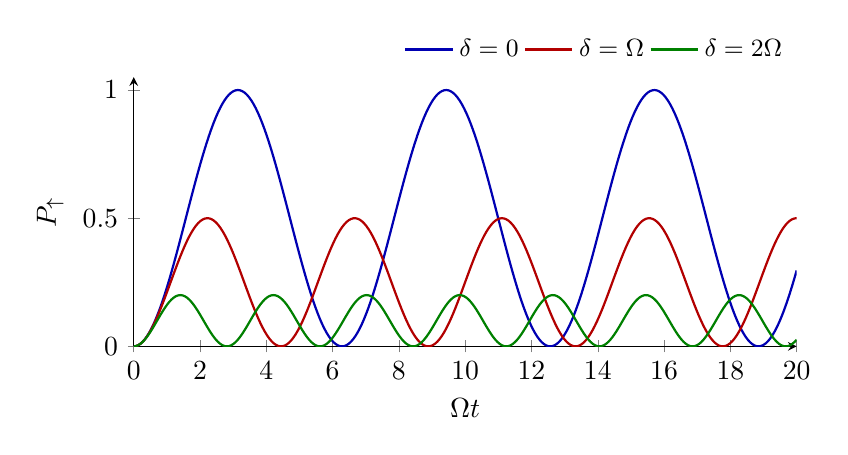
\begin{tikzpicture}
\begin{axis}[width=10cm,height=5cm,xlabel={$\Omega t$},ylabel={$P_\uparrow$},axis lines=left,xmin=0,xmax=20,ymin=0,ymax=1.05,domain=0:20,samples=300,legend style={draw=none,font=\small,at={(1,1.02)},anchor=south east,legend columns=3}]
\addplot[thick,blue!70!black]{sin(deg(x/2))^2}; \addlegendentry{$\delta=0$}
\addplot[thick,red!70!black]{(1/2)*sin(deg(sqrt(2)*x/2))^2}; \addlegendentry{$\delta=\Omega$}
\addplot[thick,green!50!black]{(1/5)*sin(deg(sqrt(5)*x/2))^2}; \addlegendentry{$\delta=2\Omega$}
\end{axis}
\end{tikzpicture}
\caption{Rabi oscillations. A $\pi$-pulse ($\Omega t = \pi$) on resonance flips the state completely; detuning reduces the maximum transfer.}
\end{figure}

The maser corresponds to $\Omega = 2\mu\mathcal{E}_0/\hbar$ and NMR to $\Omega = \gamma B_1$, $\delta = \omega-\gamma B_0$. A ``$\pi/2$ pulse'' ($\Omega t = \pi/2$) creates an equal superposition; a ``$\pi$ pulse'' inverts the populations. These are the basic single-qubit gates of quantum computing.

% ============================================================
\section{The Ammonia Molecule and the Maser}
% ============================================================

NH$_3$ is a flattened tetrahedron, with the nitrogen either above or below the plane of hydrogens: states $|{\uparrow}\rangle$ and $|{\downarrow}\rangle$. Its electronic, vibrational and rotational excitations cost much more energy and can be ignored. Classically the two configurations are degenerate minima of a double-well potential, separated by a barrier. With an infinite barrier, $\hat{H}_0 = E_0I$ in this basis. Tunnelling makes $\langle{\downarrow}|\hat{H}|{\uparrow}\rangle\neq0$; taking it real,
\[
    \hat{H}_0 = \begin{pmatrix}E_0 & -\Delta\\ -\Delta & E_0\end{pmatrix} = E_0I - \Delta\sigma_1 .
\]
\begin{figure}[ht]
\centering
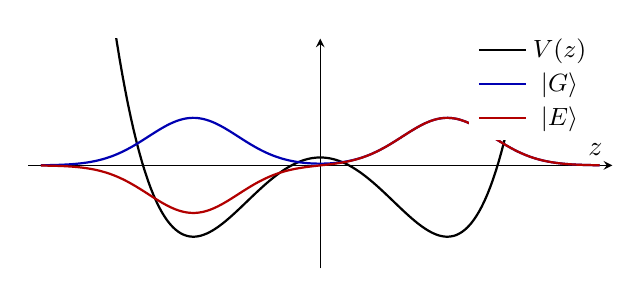
\begin{tikzpicture}
\begin{axis}[width=9cm,height=4.5cm,axis lines=middle,xlabel={$z$},ytick=\empty,xtick=\empty,xmin=-2.3,xmax=2.3,ymin=-1.3,ymax=1.6,samples=200,legend style={draw=none,at={(0.98,1.05)},anchor=north east,font=\small}]
\addplot[thick,black,domain=-2.2:2.2]{(x^2-1)^2-0.9};
\addlegendentry{$V(z)$}
\addplot[thick,blue!70!black,domain=-2.2:2.2]{0.6*(exp(-4*(x-1)^2)+exp(-4*(x+1)^2))};
\addlegendentry{$|G\rangle$}
\addplot[thick,red!70!black,domain=-2.2:2.2]{0.6*(exp(-4*(x-1)^2)-exp(-4*(x+1)^2))};
\addlegendentry{$|E\rangle$}
\end{axis}
\end{tikzpicture}
\caption{The ammonia double well. Tunnelling mixes the localized states; the symmetric combination $|G\rangle$ lies $2\Delta$ below the antisymmetric $|E\rangle$.}
\end{figure}

The eigenstates are the symmetric ground state $|G\rangle = \frac{1}{\sqrt2}(|{\uparrow}\rangle + |{\downarrow}\rangle)$ with $E_0-\Delta$, and the antisymmetric excited state $|E\rangle = \frac{1}{\sqrt2}(|{\uparrow}\rangle - |{\downarrow}\rangle)$ with $E_0+\Delta$. A molecule starting in $|{\uparrow}\rangle$ oscillates between the wells:
\[
    P_\uparrow(t) = \cos^2\frac{\Delta t}{\hbar},
    \qquad
    P_\downarrow(t) = \sin^2\frac{\Delta t}{\hbar}.
\]
Experimentally $2\Delta = 0.9782\times10^{-4}$\,eV, a microwave photon of $\nu = 23.87$\,GHz ($\lambda = 1.26$\,cm).

\paragraph{In an electric field.} Ammonia has an electric dipole moment $\bm{\mu}_E = -\mu\hat{z}$, adding $\delta\hat{H} = -\bm{\mu}_E\cdot\vect{\mathcal{E}} = \mu\mathcal{E}\sigma_3$:
\[
    \hat{H} = E_0I - \Delta\sigma_1 + \mu\mathcal{E}\sigma_3,
    \qquad
    E_{E,G} = E_0\pm\sqrt{\Delta^2 + \mu^2\mathcal{E}^2}.
\]
For weak fields $E_{E,G}\approx E_0\pm(\Delta + \mu^2\mathcal{E}^2/2\Delta)$, and for strong fields $E_{E,G}\approx E_0\pm\mu\mathcal{E}$. In a field gradient, $|G\rangle$ molecules move toward strong field and $|E\rangle$ molecules toward weak field, splitting a beam into its two energy eigenstates.

\begin{figure}[ht]
\centering
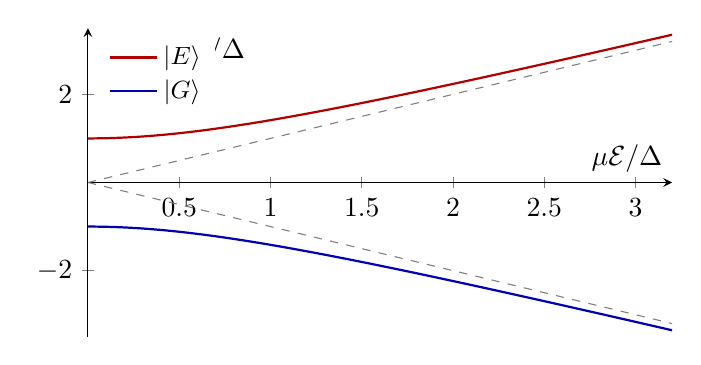
\begin{tikzpicture}
\begin{axis}[width=9cm,height=5.5cm,xlabel={$\mu\mathcal{E}/\Delta$},ylabel={$(E-E_0)/\Delta$},axis lines=middle,xmin=0,xmax=3.2,ymin=-3.5,ymax=3.5,samples=100,domain=0:3.2,legend style={draw=none,at={(0.02,0.98)},anchor=north west,font=\small}]
\addplot[thick,red!70!black]{sqrt(1+x^2)}; \addlegendentry{$|E\rangle$}
\addplot[thick,blue!70!black]{-sqrt(1+x^2)}; \addlegendentry{$|G\rangle$}
\addplot[dashed,gray]{x}; \addplot[dashed,gray]{-x};
\end{axis}
\end{tikzpicture}
\caption{Energies of ammonia in an electric field: an avoided crossing. Without tunnelling the levels $\pm\mu\mathcal{E}$ (dashed) would cross at zero field; the coupling $\Delta$ makes them repel, quadratically at weak field and linearly at strong field.}
\end{figure}

\begin{proof}[Eigenvalues of the general two-level Hamiltonian]
For $\hat{H} = g_0I + \lvect{g}\cdot\bm{\sigma}$, $(\lvect{g}\cdot\bm{\sigma})^2 = |\lvect{g}|^2I$, so the eigenvalues of $\lvect{g}\cdot\bm{\sigma}$ square to $|\lvect{g}|^2$ and, being traceless, are $\pm|\lvect{g}|$. Here $\lvect{g} = (-\Delta,0,\mu\mathcal{E})$, so $E = E_0\pm\sqrt{\Delta^2+\mu^2\mathcal{E}^2}$, and the eigenvectors are the spin states along $\uvect{g}$, with polar angle $\tan\theta = \Delta/\mu\mathcal{E}$ and azimuth $\varphi = \pi$.
\end{proof}

\paragraph{The maser.} Pass the $|E\rangle$ beam through a cavity with an oscillating field $\mathcal{E}(t) = 2\mathcal{E}_0\cos\omega_0t$ tuned to resonance, $\omega_0 = 2\Delta/\hbar$. In the $\{|E\rangle,|G\rangle\}$ basis, $\hat{H} = \begin{pmatrix}\Delta & \mu\mathcal{E}\\ \mu\mathcal{E} & -\Delta\end{pmatrix}$ (dropping $E_0$). Writing $C_E = e^{-i\Delta t/\hbar}B_E$ and $C_G = e^{i\Delta t/\hbar}B_G$,
\[
    \frac{d}{dt}\begin{pmatrix}B_E\\B_G\end{pmatrix} = -\frac{i\mu\mathcal{E}_0}{\hbar}\begin{pmatrix}0 & 1+e^{2i\omega_0t}\\ 1+e^{-2i\omega_0t} & 0\end{pmatrix}\begin{pmatrix}B_E\\B_G\end{pmatrix}.
\]
For $\mu\mathcal{E}_0\ll\Delta$, $B_{E,G}$ vary slowly, so the rapidly oscillating terms average to zero (the \emph{rotating-wave approximation}). Then
\[
    B_E(t) = \cos\frac{\mu\mathcal{E}_0t}{\hbar},
    \qquad
    B_G(t) = -i\sin\frac{\mu\mathcal{E}_0t}{\hbar},
    \qquad
    P_E(t) = \cos^2\frac{\mu\mathcal{E}_0t}{\hbar}.
\]
If each molecule spends $T = \frac{\hbar}{\mu\mathcal{E}_0}\frac\pi2(2n+1)$ in the cavity, it leaves in $|G\rangle$, having deposited a photon of energy $2\Delta$ into the field. This builds up a coherent single-mode field: microwave amplification by stimulated emission of radiation (Townes, Gordon and Zeiger, 1953). Ammonia masers were the first atomic clocks, and also occur naturally in astrophysics.

% ============================================================
\section{Neutrino Oscillations}
% ============================================================

Neutrinos are produced and detected in \emph{flavour} states ($\nu_e$, $\nu_\mu$), but propagate in \emph{mass} eigenstates $\nu_1$, $\nu_2$ with masses $m_1\neq m_2$. In a two-flavour model these are related by a rotation:
\[
    |\nu_e\rangle = \cos\theta|\nu_1\rangle + \sin\theta|\nu_2\rangle,
    \qquad
    |\nu_\mu\rangle = -\sin\theta|\nu_1\rangle + \cos\theta|\nu_2\rangle .
\]
For an ultrarelativistic neutrino of momentum $p$, $E_i = \sqrt{p^2c^2+m_i^2c^4}\approx pc + m_i^2c^3/2p$, so after a time $t = L/c$ the relative phase between the mass states is $(E_2-E_1)t/\hbar = \Delta m^2c^3L/2p\hbar c$. Then
\[
    P(\nu_e\to\nu_\mu) = |\langle\nu_\mu|\Psi(t)\rangle|^2 = \sin^22\theta\,\sin^2\Bigl(\frac{\Delta m^2c^4L}{4\hbar cE}\Bigr).
\]
This is the same algebra as the ammonia molecule, with a ``mixing angle'' $\theta$ that is not $\pi/4$. The observation of such oscillations (solar and atmospheric neutrinos) proved that neutrinos have mass (Nobel Prize, 2015).

% ============================================================
\section{Nuclear Magnetic Resonance}
% ============================================================

Consider a spin-$\frac12$ particle in a static field along $\hat{z}$ plus a circularly polarized RF field:
\[
    \vect{B}(t) = B_0\khat + B_1(\cos\omega t\,\ihat - \sin\omega t\,\jhat),
    \qquad
    \hat{H}(t) = -\gamma\bigl(B_0\hat{S}_z + B_1\cos\omega t\,\hat{S}_x - B_1\sin\omega t\,\hat{S}_y\bigr).
\]
Now $[\hat{H}(t_1),\hat{H}(t_2)]\neq0$. Rather than a time-ordered exponential, transform to a rotating frame. One shows (by differentiating $f(\theta) = e^{i\theta\sigma_3}\sigma_1e^{-i\theta\sigma_3}$ twice, giving $f'' = -4f$) that
\[
    \cos\omega t\,\hat{S}_x - \sin\omega t\,\hat{S}_y = e^{i\omega t\hat{S}_z/\hbar}\hat{S}_xe^{-i\omega t\hat{S}_z/\hbar}.
\]
In terms of the rotating-frame state $|\Psi_R,t\rangle = e^{-i\omega t\hat{S}_z/\hbar}|\Psi,t\rangle$, the Hamiltonian becomes time-independent:
\[
    i\hbar\frac{d}{dt}|\Psi_R,t\rangle = \bigl[(\omega-\gamma B_0)\hat{S}_z - \gamma B_1\hat{S}_x\bigr]|\Psi_R,t\rangle = -\gamma\vect{B}_{\text{eff}}\cdot\hat{\lvect{S}}\,|\Psi_R,t\rangle,
    \qquad
    \vect{B}_{\text{eff}} = \Bigl(B_0-\frac\omega\gamma\Bigr)\khat + B_1\ihat .
\]

\begin{formula}[NMR solution]
\[
    |\Psi,t\rangle = e^{i\omega t\hat{S}_z/\hbar}\,e^{i\gamma\vect{B}_{\text{eff}}\cdot\hat{\lvect{S}}t/\hbar}\,|\Psi,0\rangle .
\]
\end{formula}

Take $B_0\gg B_1$ and $|\Psi,0\rangle = |\hat{z},+\rangle$. Off resonance, $\vect{B}_{\text{eff}}\approx\hat{z}$ and nothing happens. On resonance, $\omega = \omega_0 = \gamma B_0$, $\vect{B}_{\text{eff}} = B_1\ihat$, and the spin precesses about the rotating $x$-axis; after $\Delta t = \pi/2\gamma B_1$ (a ``$90^\circ$ pulse'') it points along the rotating $y$-axis. Switching off $B_1$ leaves it precessing rapidly in the $xy$-plane. In the lab frame the spin spirals slowly from the $z$-axis down into the $xy$-plane while precessing rapidly about $z$.

\begin{figure}[ht]
\centering
\begin{tikzpicture}[>=Stealth,scale=1.3]
  \draw[->] (0,0) -- (0,2.2) node[above]{$z$};
  \draw[->] (0,0) -- (2.2,0) node[right]{$y$};
  \draw[->] (0,0) -- (-1.1,-0.7) node[below left]{$x$};
  \draw[thick,blue!70!black,domain=0:12.56,samples=300,smooth,variable=\t] plot ({1.6*sin(deg(\t/8))*sin(deg(3*\t))*0.9 + 0.0},{1.6*cos(deg(\t/8))*1.0 + 0.35*1.6*sin(deg(\t/8))*cos(deg(3*\t))});
  \node[blue!70!black] at (1.9,1.6) {\small spin path};
\end{tikzpicture}
\caption{NMR in the lab frame during a $90^\circ$ pulse: the spin spirals from the $z$-axis down to the $xy$-plane while precessing rapidly about $z$.}
\end{figure}

\paragraph{Relaxation.} Real spins interact with their surroundings. Phenomenologically, the polarization $\lvect{M}$ (the Bloch vector of the ensemble) obeys the \emph{Bloch equations}
\[
    \dot{M}_{x,y} = \bigl(\gamma\lvect{M}\times\vect{B}\bigr)_{x,y} - \frac{M_{x,y}}{T_2},
    \qquad
    \dot{M}_z = \bigl(\gamma\lvect{M}\times\vect{B}\bigr)_z - \frac{M_z - M_0}{T_1},
\]
where $T_1$ (longitudinal relaxation) is the time to re-establish thermal polarization $M_0$ along $\vect{B}$, and $T_2\le2T_1$ (transverse relaxation) the time for the precessing spins to dephase. In density-matrix language, $T_1$ relaxes the populations and $T_2$ kills the coherences: decoherence (Chapter~\ref{ch:density}). Different tissues have different $T_1$ and $T_2$, which provides MRI's contrast.

\begin{fact}[Magnetic resonance imaging]
The body is mostly water, so mostly protons, which are spin-$\frac12$. A large static field $B_0\approx2$\,T aligns the spins along $\hat{z}$. A $90^\circ$ pulse with $B_1\sim0.01$\,T sets them rotating in the $xy$-plane at the Larmor frequency, and the rotating dipoles emit a radio-frequency signal picked up by receiver coils. The signal locates the protons, and its decay time, set by interactions between spins, distinguishes tissues. NMR is also used to study materials and to manipulate qubits.
\end{fact}

\begin{fact}[Spin and spin statistics]
Spin is an intrinsic angular momentum: it obeys the same algebra as $\hat{\lvect{L}}$, and total angular momentum (orbital plus spin) is conserved, but it can be half-integer and has no spatial wavefunction. Particles with half-integer spin are \emph{fermions}; those with integer spin are \emph{bosons}. Including spin, a hydrogen eigenstate is $|n,\ell,m,s\rangle$, with degeneracy $2n^2$.
\end{fact}

\begin{fact}[Key results of this chapter]
\leavevmode
\begin{itemize}
\item Every two-state Hamiltonian is $g_0I + \lvect{g}\cdot\bm{\sigma}$, with energies $g_0\pm|\lvect{g}|$.
\item Spin states $|\uvect{n},\pm\rangle$ live on the Bloch sphere; rotations $e^{-i\alpha\uvect{n}\cdot\bm{\sigma}/2}$ have half-angles.
\item Spins precess at the Larmor frequency; tunnelling splits ammonia's levels by $2\Delta$.
\item Driven systems undergo Rabi oscillations, $P = \frac{\Omega^2}{\Omega_R^2}\sin^2\frac{\Omega_Rt}{2}$: masers, NMR, MRI, qubit gates.
\end{itemize}
\end{fact}
